\documentclass[12pt, titlepage]{article}

\usepackage{booktabs}
\usepackage{tabularx}
\usepackage{hyperref}
\usepackage{color}
\usepackage{geometry}
\usepackage{amsmath}
\usepackage{graphicx}
\hypersetup{
    colorlinks,
    citecolor=black,
    filecolor=black,
    linkcolor=red,
    urlcolor=blue
}
\usepackage[round]{natbib}


\title{SE 3XA3: Test Report\\Asteroid War Game}

\author{Team 12, 3XA3-Lab3-Group12
		\\ Student 1 Eric Thai Thaie1
		\\ Student 2 Tianzheng Mai and mait6
		\\ Student 3 Linqi Jiang and jiangl21
		\\ Student 4 Junhong Chen and chenj297
}

\date{\today}

\begin{document}
\maketitle
\section* {Overview}
The game is implemented by Javascript and is executed on a browser. The requirement for the user is a keyboard for game operation, a mouse to select different activities, Internet and browser to access the game. The goal of the game is to reach the score as high as possible by destroying asteroids. The User interface contains four buttons with different functionalities and the project title "\textcolor{red}{Welcome to 3XA3 L03 Group 12 Project}", the team members' names are displayed below the title. \textcolor{red}{ONE PLAYER MODE} will guide the user to the game of Aesteriod with one-player-mode.\textcolor{red}{TWO PLAYER MODE} will guide the user to the game of Aesteriod with a two-player mode. \textcolor{red}{USER MANUAL} will guide the user to the help page which contains the game rules and operation methods. \textcolor{red}{CONTACT US} will guide the user to the page that contains the information of the team members.

\begin{figure}[!h]
\begin{center}

\includegraphics[width=0.8\textwidth]{MainPage.jpg}
\end{center}
\caption{MainPage}
\label{fig:Main_Pager}
\end{figure}

\begin{figure}[!h]
\begin{center}
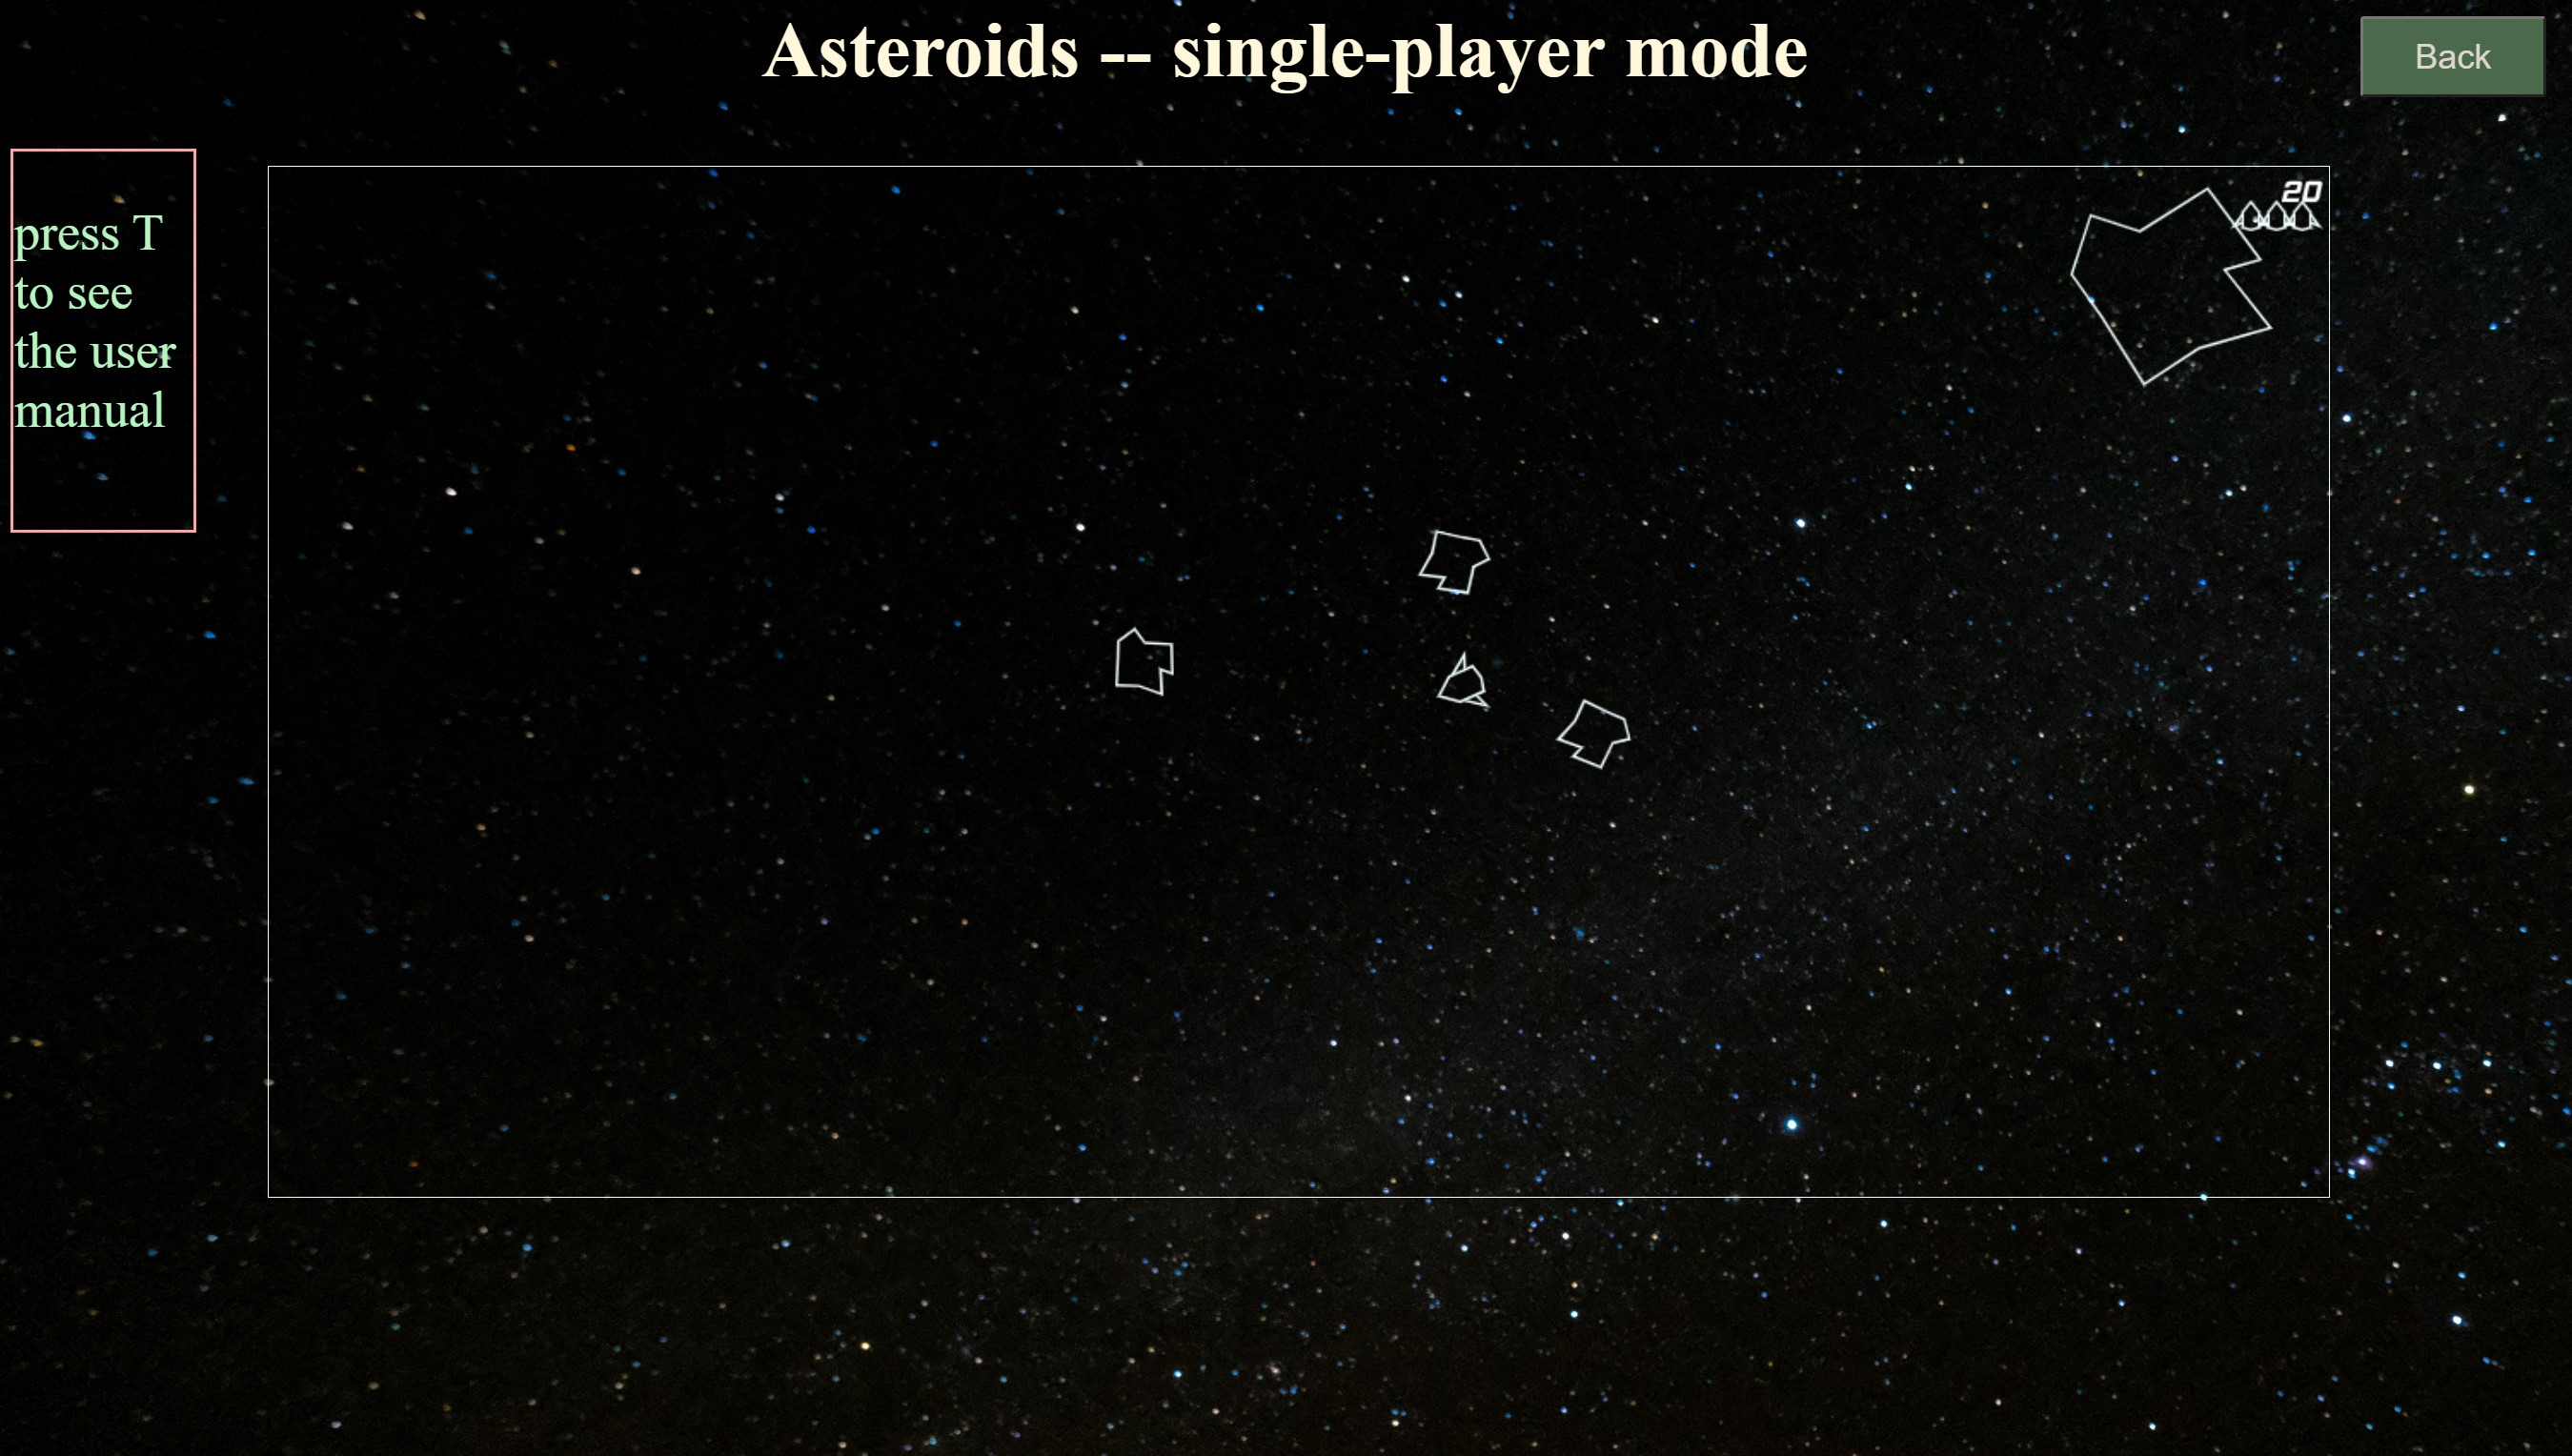
\includegraphics[width=0.8\textwidth]{One_Player_Mode.jpg}
\end{center}
\caption{One Player Mode}
\label{fig:single_Player}
\end{figure}

\begin{figure}[!h]
\begin{center}
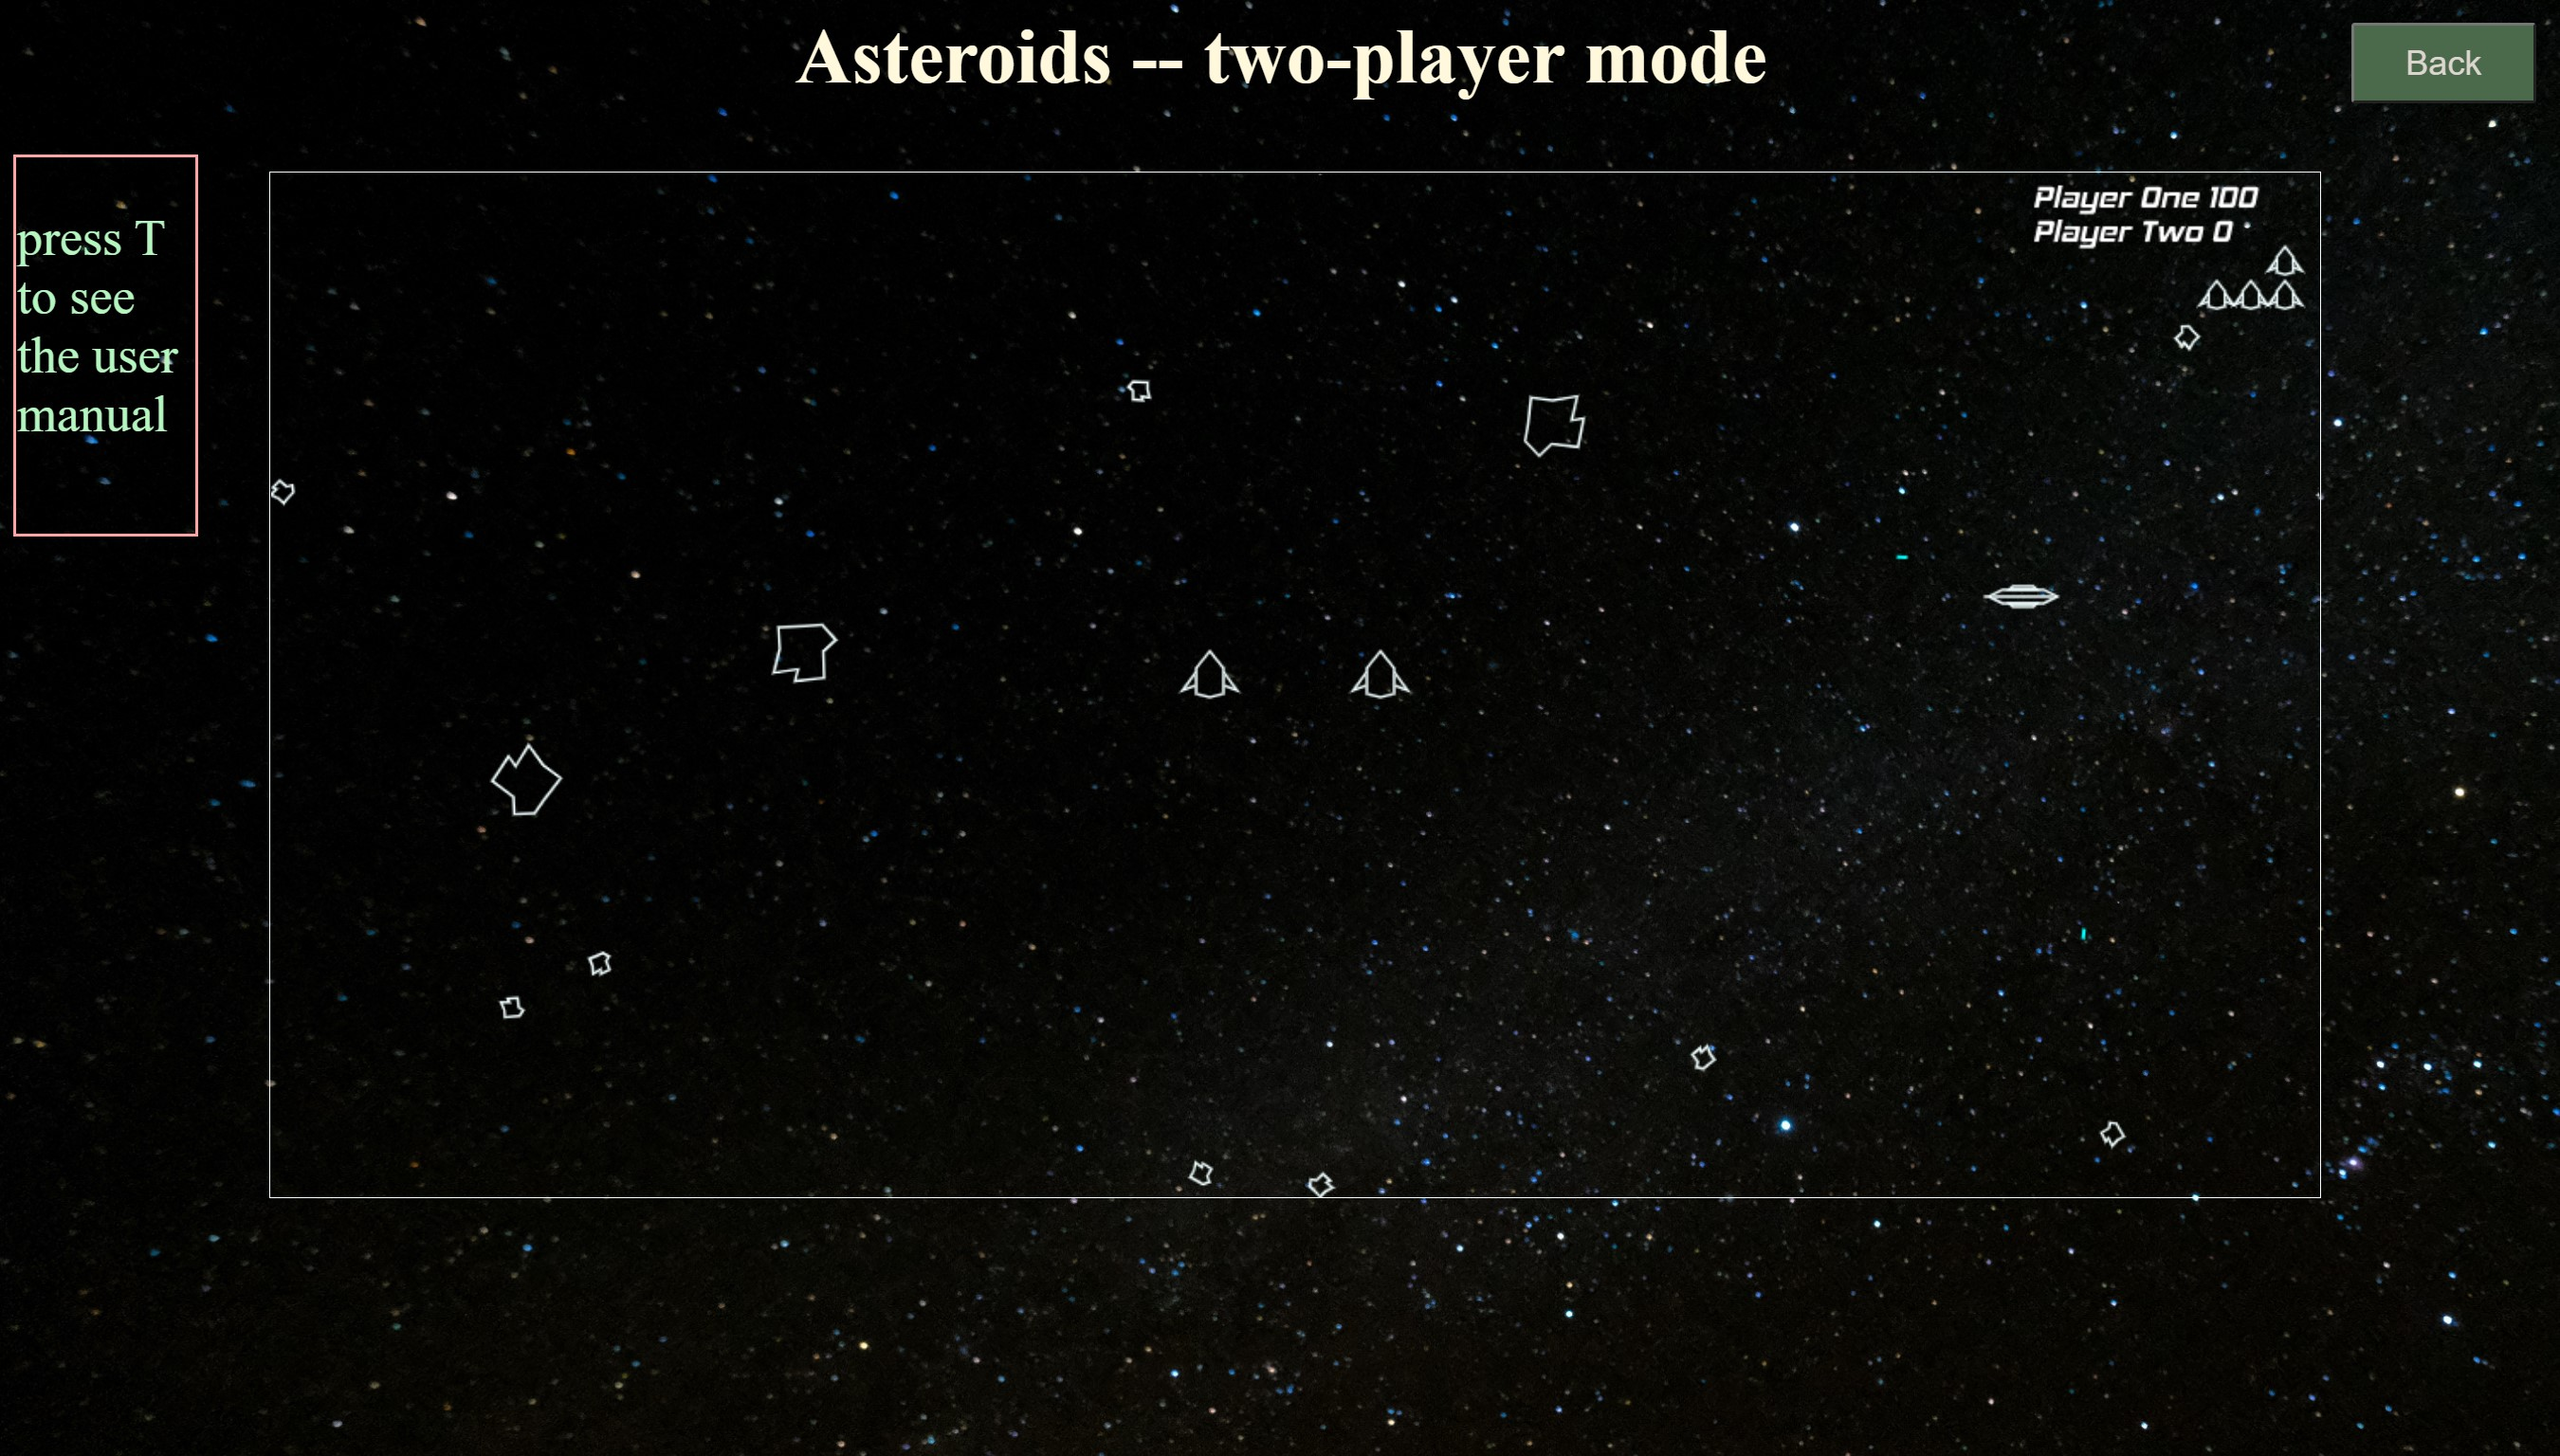
\includegraphics[width=0.8\textwidth]{Two_Player_Mode.jpg}
\end{center}
\caption{Two Player Mode}
\label{fig:two_Players}
\end{figure}

\section* {Game description}
In One-player mode, the user will control exactly one spaceship to destroy the asteroids by firing bullets. The biggest Asteroid will split into three small ones after collision and UFO will appear randomly to fire at the user's ship. Each user has three lives, hit by the asteroid or destroyed by UFO will lose one life. The game will over if all the lives are lost. Score and lives left will be illustrated on the right top corner, the user can also press T to open the help page. In two-player mode, there will be two ships controlled by different keys by users. Both ship information will be displayed on the right top corner as well and the game will over if two ships run out of lives. Both modes will display the final score of the users when the game is over and contain a back button to return to the home page.
\section* {Game operation}
The ship is controlled by key arrows in one-player mode, the ship will move according to the key arrows input, space is used for fire bullets. Also, in two-player mode, keys WSAD will be used to control the second ship movement and shift is used to fire bullets. Detailed operation methods are specified in the USER MANUAL.
\end{document}